%
% modest-design.tex
% Time-stamp: <2006-05-12 18:47:13 (djcb)>
%
\documentclass{book}
\usepackage{graphics}

% macros
\newcommand{\modest}{{\tt modest} } 
\newcommand{\tinymail}{{\tt tinymail} }
\newcommand{\camel}{{\tt libcamel} }

\newcommand{\djcbemail}{$<$dirk-jan.binnema@nokia.com$>$ }
\newcommand{\smtp}{{\sc SMTP} }
\newcommand{\pop}{{\sc POP3} }
\newcommand{\imap}{{\sc IMAP} }
\newcommand{\gtk}{{\sc GTK+} }
\newcommand{\gconf}{{\sc GConf} }

\author{Dirk-Jan C. Binnema\\\djcbemail}
\title{{\huge \modest}\\
an e-mail program for small devices\\
architecture \& design}
\setlength{\parskip}{8pt}
\setlength{\parindent}{0pt}
\begin{document}
\maketitle
\tableofcontents
\chapter*{Introduction}
\modest is a mail user agent (MUA) targetting small devices, in particular
Nokia's {\em Nokia 770 Internet Tablet}. This document describes the design
and implementation of this software.

\modest lives at the top of a extensive stack of software. It is built on
top of {\tt libtinymail}, and uses its libcamel backend. It strives to the be
a simple yet powerful program, geared towards small devices, for example (but
not limited to) Nokia's 770 internet tablet. An important goal is to minimize
memory usage while still being able to handle significant amounts of email
quickly; much of that is achieved simply by using \tinymail, which
uses a number of clever tricks for that, such as the proxy design pattern for
listing email headers, and not needing memory for headers which are not
currently visible.

\modest, in turn, also tries to be efficient, fast and {\em scalable}. That
means that the MUA should support multiple user-interfaces, perhaps making it
even possible to switch between them during runtime. 

To summarize the goals for \modest:
\begin{itemize}
\item target devices with limited amounts of memory ("limited" in 2006 terms means
  less than 64Mb, and of which only part can be used for e-mail);
\item target Linux/Unix-like environments with GLib/GTK+-based support;
\item support multiple user-interface (UIs) with as
  much code sharing as possible between the different UIs.
\end{itemize}

Like {\tt libtinymail} and {\tt libcamel}, \modest is programmed in C, using the
GObject-system for object-oriented (OO) features. For now, it specifically
targets \gtk based UIs (and derivatives like "Hildon"). 

\chapter{Architecture}
\modest tries to be quite flexible in its design. However, it's always
important not to make things {\em too} generic. Both for reasons of time
limitations and keeping the software understandable and ``modest'', it's
important to limit the scope.

For \modest, the following:
\begin{itemize}
  \item \modest is a e-mail program using the \tinymail and \camel libraries;
  \item \modest targets \gtk and \gconf-based user-interfaces, including the Hildon
    environment;
  \item \modest main use-case is in small, mobile device such as Nokia's {\em 770
    Internet Tablet};
  \item However, effort is made also to make \modest usable as a
    general-purpose e-mail client on normal desktop computer.
\end{itemize}


\chapter{Design}
In this chapter, we'll discuss the design of various parts of \modest. We'll
not go into the details of various APIs. Please consult the documentation
generated from the source code ({\tt gtk-doc}) for that.

There are {\tt \#define}-definitions for many account keys in {\tt
  modest-account-keys.h}. 

\section {Configuration}
Configuration is the part of \modest that deals with storing all
settings. While the design allows for alternative implementations, currently
only {\tt gconf} is supported as a backend.

All dealing with configuration is done with the {\tt ModestConf} GObject. This
object is declared in {\tt modest-conf.h}, and the GConf-based implementation in
{\tt modest-conf-gconf.c}. As said, there could be different implementations
{\tt modest-conf-myconf.c}, but we use the GConf-backed system. However,
nothing GConf-specific is visible in the ModestConf API.

\section{Account Management}
Account Management is the part of \modest that deals with the setting related
to sending and receiving of e-mail. We will follow the libcamel-convention of
using the term {\em store} for a e-mail storage/retrieval server, and a {\em
  transport} for a server that transports mail to its destination.

In practice, the following types are available:
\begin{itemize}
  \item {\bf stores}: \pop and \imap;
  \item {\bf transports}: {\tt sendmail} and \smtp.
\end{itemize}

\subsection{Definitions}
\begin{itemize}
    \item An {\bf account} is a named entity consisting of a {\bf store} and a
    {\bf transport}.\footnote{For our mobile use-cases, the {\em transport}
      cannot be a static entity, but may depend on the network
      connection. That is however not part of Account Management, so not
      discussed here}
    \item  A {\bf server account} is account describing the connection with a
      specific server. Server accounts come in two type:
      \begin{itemize}
      \item A {\bf transport} describes the connection information (servername,
        username, password etc.) for a transport server;
      \item A {\bf store} describes the connection information for a store server;
      \end{itemize}
\end{itemize}

\subsection{Code}
The functions to deal with account and server accounts are located in {\tt
  ModestAccountMgr}, ie. in {\tt modest-account-mgr.[ch]}. There function to
add specific values for both, to list the available ones, etc. Please refer to
the source code documentation for details.

\subsection{Location in configuration database}
{\em Accounts} can be found in {\tt /apps/modest/accounts}, while {\em server
  accounts} can be found in {\tt /app/modest/server\_accounts}.

The following image show an account {\em accountstest} with server accounts
{\tt mystore} and {\tt mytransport}.

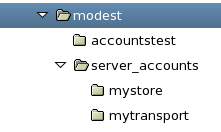
\includegraphics{modest-account-mgr.png}

For each of the stores, there are number of parameters specified:
\begin{itemize}
\item {\tt hostname} - the place where the server resides;
\item {\tt username} - the username;
\item {\tt password} - the password;
\item {\tt proto} - the protocal for communication with this server - for
  now these are the following valid values (literal strings):
  \begin{itemize}
  \item {\tt sendmail};
  \item {\tt smtp};
  \item {\tt pop}
  \item {\tt imap}.
  \end{itemize}
\end{itemize}

In the {\tt modest-proto.[ch]} there are various functions to check whether
something is a valid protocol, and whether it is a transport of a store. 

Note that server accounts and accounts are relatively independent. While
accounts refer to two server accounts, these server accounts can be
used by other accounts as well.

The reason two keep accounts and server accounts separately, is a bit of
flexibility. In mobile use-cases, quite often it's desirable to use a
network-specific smtp-server. The chosen structure makes it easy to iterate
over all smtp-servers and find the right one.

\chapter{Finding the Transport}
One of the interesting topics in designing a mobile e-mail client is to deal
with transports (in particular, \smtp). The reason for that is that the
majority of \smtp-servers only allow e-mail from the same network. That means
that for example {\tt smtp.some-isp.com} will only accept mail from ({\tt MAIL
  FROM:}) {\tt user@some-isp.com}, and refuse mail from {\tt
  user@some-other-isp.com}, unless the recipient {\tt RCPT TO:} is on the same
network. 

To summarize:

\footnote{Some smtp-servers {\bf will} accept mail
  from} 



\chapter*{Coding guidelines}
When hacking on \modest, please honour these time-tested coding guidelines.
First, please follow the {\em Linux CodingStyle guidelines}:\\
       {\tt /usr/src/linux/Documentation/CodingStyle}\\
Then, read the {\em OSSO Coding Style Guidelines}:\\
        {\tt http://foo}
Here are only some additional notes.

Your editor may help you with this, for example for {\tt emacs}:
\begin{verbatim}
  (c-set-style "K&R")
  (setq tab-width 8)
  (setq indent-tabs-mode t)
  (setq c-basic-offset 8)
\end{verbatim}

Or the equivalent in your favourite editor.

Lines should not exceed 100 characters.

Global functions (the ones in {\tt .h}-files) should be commented using 
doxygen-style comments.

Furthermore, please follow 'conventional wisdom' for programming with 
GLib/GTK+/GObject. Some things to remember:
\begin{itemize}
\item {\tt g\_new}, {\tt g\_malloc} and friends {\bf never} return {\tt NULL}. They terminate
  the application if it happens (normally). No need to check for {\tt NULL} returns.
\item {\tt g\_return\_if\_fail} and friends may be 'turned off', ie. they are
  to be used for error checking, but {\bf not} for your programming logic
\end{itemize}

To test for the validity of function parameters,
%   g_return_if_fail / g_return_val_if_fail

ie.
\begin{verbatim}
double
one_divided_by_x (double x)
{
        g_return_val_if_fail ((x != 0), -1);
        return 1/x;     
}
\end{verbatim}
This will give us a warning (and a wrong answer) in case we do
%     one_divided_by_x (0);

This is good for testing, but it's important to keep in mind that in
production code the check may be turned off. The caller should make
sure that the parameter is correct (ie. != 0 in this case).

Now, if a similar check is actually part of the logic of a function,
then {\tt g\_return\_if\_fail} should not be used, but instead, e.g.:
\begin{verbatim}
int
stack_item_num (Stack *stack)
{
        if (!stack)
                return 0;

        /* calculate item count */
}
\end{verbatim}
\end{document}
